

\section*{ID: 3c8fdc40}
A printer produces posters at a constant rate of 42 posters per minute. At what rate, in posters per hour, does the printer produce the posters?

\section*{ID: d28c29e1}
The International Space Station orbits Earth at an average speed of 4.76 miles per second. What is the space station's average speed in miles per hour?\\
A. 285.6\\
B. 571.2\\
C. 856.8\\
D. $17,136.0$

\section*{ID: 3f5398a6}
For a person $m$ miles from a flash of lightning, the length of the time interval from the moment the person sees the lightning to the moment the person hears the thunder is $k$ seconds. The ratio of $m$ to $k$ can be estimated to be 1 to 5 . According to this estimate, the person is how many miles from a flash of lightning if the time interval is 25 seconds?\\
A. 10\\
B. 9\\
C. 6\\
D. 5

\section*{ID: b4912cc5}
The population density of Iceland, in people per square kilometer of land area, increased from 2.5 in 1990 to 3.3 in 2014. During this time period, the land area of Iceland was 100,250 square kilometers. By how many people did Iceland's population increase from 1990 to 2014?\\
A. 330,825\\
B. 132,330\\
C. 125,312\\
D. 80,200

A customer spent $\$ 27$ to purchase oranges at $\$ 3$ per pound. How many pounds of oranges did the customer purchase?

\section*{ID: 000259aa}
A group of monarch butterflies migrated from Chicago, Illinois, to Michoacán, Mexico, flying a total of 2,100 miles. It took a single butterfly in the group 120 days to travel this route one way. On average, how many miles did the butterfly travel per day?\\
A. 0.057\\
B. 0.729\\
C. 17.5\\
D. 24

ID: 3726e079

If $\frac{x}{y}=4$ and $\frac{24 x}{n y}=4$, what is the value of $n$ ?

In a box of pens, the ratio of black pens to red pens is 8 to 1 . There are 40 black pens in the box. How many red pens are in the box?\\
A. 5\\
B. 8\\
C. 40\\
D. 320

\section*{ID: 8e528129}
Pure beeswax has a density of 0.555 ounce per cubic inch. An online company sells pure beeswax at a price of $\$ 8.00$ per ounce. What is the selling price, in dollars per cubic inch, for pure beeswax purchased from this company?

\section*{ID: 15617f62}
The population density of Worthington is 290 people per square mile. Worthington has a population of 92,800 people. What is the area, in square miles, of Worthington?\\
A. 102,400\\
B. 93,090\\
C. 320\\
D. 32






















































Jeremy deposited $x$ dollars in his investment account on January 1, 2001. The amount of money in the account doubled each year until Jeremy had 480 dollars in his investment account on January 1, 2005. What is the value of $x$ ?

\section*{ID: 445 dd 032}
Tanya earns $\$ 13.50$ per hour at her part-time job. When she works $z$ hours, she earns $13.50 z$ dollars. Which of the following expressions gives the amount, in dollars, Tanya will earn if she works $3 z$ hours?\\
A. $3(13.50 z)$\\
B. $3+13.50 z$\\
C. $3 z+13.50 z$\\
D. $13.50(z+3)$

\section*{ID: fe1ec415}
A cherry pitting machine pits 12 pounds of cherries in 3 minutes. At this rate, how many minutes does it take the machine to pit 96 pounds of cherries?\\
A. 8\\
B. 15\\
C. 24\\
D. 36

\section*{ID: ba62b0b0}
A kangaroo has a mass of 28 kilograms. What is the kangaroo's mass, in grams? ( 1 kilogram $=1,000$ grams)\\
A. 28,000\\
B. 1,028\\
C. 972\\
D. 784\\
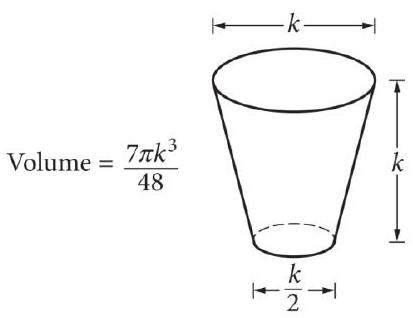
\includegraphics[max width=\textwidth, center]{2025_06_15_a366e2a72ef746fddc1dg-25}

The glass pictured above can hold a maximum volume of 473 cubic centimeters, which is approximately 16 fluid ounces. Jenny has a pitcher that contains 1 gallon of water. How many times could Jenny completely fill the glass with 1 gallon of water? (1 gallon=128 fluid ounces)\\
A. 16\\
B. 8\\
C. 4\\
D. 3

\section*{ID: 7cd1c6db}
An object travels at a constant speed of 12 centimeters per second. At this speed, what is the time, in seconds, that it would take for the object to travel 108 centimeters?\\
A. 9\\
B. 96\\
C. 120\\
D. 972

\begin{center}
\begin{tabular}{|l|l|l|l|l|}
\hline
\multirow{2}{*}{State} & \multicolumn{4}{|c|}{Power capacity} \\
\hline
 & Low & Medium & High & Total \\
\hline
Texas & 4 & 2 & 3 & 9 \\
\hline
California & 1 & 0 & 1 & 2 \\
\hline
Oregon & 1 & 0 & 1 & 2 \\
\hline
Indiana & 0 & 2 & 0 & 2 \\
\hline
Colorado & 1 & 1 & 0 & 2 \\
\hline
lowa & 2 & 0 & 0 & 2 \\
\hline
Oklahoma & 1 & 0 & 0 & 1 \\
\hline
Total & 10 & 5 & 5 & 20 \\
\hline
\end{tabular}
\end{center}

The table shows the distribution, by location and power capacity (maximum rate of power generation) of the twenty largest wind projects in the United States in 2013.\\
The total power capacity of the nine wind projects located in Texas was 4,952 megawatts (MW), and the total power capacity of the twenty wind projects was $11,037 \mathrm{MW}$ in 2013 . The amount of energy produced in one hour at a rate of one megawatt is one megawatt-hour. If each of the nine Texas wind projects in 2013 had operated continuously for 24 hours at the maximum rate of power generation, approximately how many megawatt-hours of energy would the nine projects have produced?\\
A. 200\\
B. 5,000\\
C. 11,000\\
D. 120,000

If $\frac{4 a}{b}=6.7$ and $\frac{a}{b n}=26.8$, what is the value of $n$ ?

The weight of an object on Venus is approximately $\frac{9}{10}$ of its weight on Earth. The weight of an object on Jupiter is approximately $\frac{23}{10}$ of its weight on Earth. If an object weighs 100 pounds on Earth, approximately how many more pounds does it weigh on Jupiter than it weighs on Venus?\\
A. 90\\
B. 111\\
C. 140\\
D. 230

\section*{ID: e21d10a7}
One of a planet's moons orbits the planet every 252 days. A second moon orbits the planet every 287 days. How many more days does it take the second moon to orbit the planet 29 times than it takes the first moon to orbit the planet 29 times?

\section*{ID: 7d721177}
The density of a certain type of wood is 353 kilograms per cubic meter. A sample of this type of wood is in the shape of a cube and has a mass of 345 kilograms. To the nearest hundredth of a meter, what is the length of one edge of this sample?\\
A. 0.98\\
B. 0.99\\
C. 1.01\\
D. 1.02

\section*{ID: d0d9ede4}
How many feet are equivalent to 34 yards? $(1$ yard $=3$ feet $)$

To make a bakery's signature chocolate muffins, a baker needs 2.5 ounces of chocolate for each muffin. How many pounds of chocolate are needed to make 48 signature chocolate muffins? (1 pound = 16 ounces)\\
A. 7.5\\
B. 10\\
C. 50.5\\
D. 120

Which of the following speeds is equivalent to 90 kilometers per hour? ( 1 kilometer = 1,000 meters)\\
A. 25 meters per second\\
B. 32 meters per second\\
C. 250 meters per second\\
D. 324 meters per second

A distance of 61 furlongs is equivalent to how many feet? ( 1 furlong $=220$ yards and 1 yard $=3$ feet)

\section*{ID: 7e6c745f}
\begin{center}
\begin{tabular}{|c|l|c|}
\hline
Food & Protein & Cost \\
\hline
1 large egg & 6 grams & $\$ 0.36$ \\
\hline
1 cup of milk & 8 grams & $\$ 0.24$ \\
\hline
\end{tabular}
\end{center}

The table above shows the amount of protein in two foods and the cost of each food. Based on the table, what is the ratio of the cost per gram of protein in a large egg to the cost per gram of protein in a cup of milk?\\
A. $1: 2$\\
B. 2 : 3\\
C. $3: 4$\\
D. $2: 1$

A fish swam a distance of 5,104 yards. How far did the fish swim, in miles? ( 1 mile $=1,760$ yards)\\
A. 0.3\\
B. 2.9\\
C. 3,344\\
D. 6,864

The population density of Cedar County is 230 people per square mile. The county has a population of 85,100 people. What is the area, in square miles, of Cedar County?

\section*{ID: 2cdefcb1}
What length, in centimeters, is equivalent to a length of 51 meters? ( 1 meter $=100$ centimeters)\\
A. 0.051\\
B. 0.51\\
C. 5,100\\
D. 51,000

\section*{ID: c7c6445f}
A certain town has an area of 4.36 square miles. What is the area, in square yards, of this town? ( 1 mile $=1,760$ yards)\\
A. 404\\
B. 7,674\\
C. 710,459\\
D. $13,505,536$

\section*{ID: 73ddfdac}
A distance of 112 furlongs is equivalent to how many feet? ( 1 furlong $=220$ yards and 1 yard $=3$ feet)

For the values $j$ and $k$, the ratio of $j$ to $k$ is 11 to 12 . If $j$ is multiplied by 17 , what is $k$ multiplied by in order to maintain the same ratio?

\section*{ID: 3ac09984}
Marta has 7,500 pesos she will convert to US dollars using a currency exchange service. At this time, the currency exchange rate is 1 peso $=0.075$ US dollars. The exchange service will charge Marta a $2 \%$ fee on the converted US dollar amount. How many US dollars will Marta receive from the currency exchange after the $2 \%$ fee is applied?\\
A. $\$ 551$\\
. 25\\
B. $\$ 562$\\
.50\\
C. $\$ 5,625$\\
. 00\\
D. $\$ 98,000$\\
. 00

How many tablespoons are equivalent to 14 teaspoons? ( 3 teaspoons $=1$ tablespoon)

A triathlon is a multisport race consisting of three different legs. A triathlon participant completed the cycling leg with an average speed of 19.700 miles per hour. What was the average speed, in yards per hour, of the participant during the cycling leg? ( 1 mile $=1,760$ yards )

\section*{ID: 551c52b9}
Tilly earns $p$ dollars for every $w$ hours of work. Which expression represents the amount of money, in dollars, Tilly earns for $39 w$ hours of work?\\
A. $39 p$\\
B. $\frac{p}{39}$\\
C. $p+39$\\
D. $p-39$

\section*{ID: 1180401d}
The total area of a coastal city is 92.1 square miles, of which 11.3 square miles is water. If the city had a population of 621,000 people in the year 2010, which of the following is closest to the population density, in people per square mile of land area, of the city at that time?\\
A. 6,740\\
B. 7,690\\
C. 55,000\\
D. 76,000

\section*{ID: f6cbb04a}
$d=55 t$

The equation above can be used to calculate the distance $d$, in miles, traveled by a car moving at a speed of 55 miles per hour over a period of $t$ hours. For any positive constant $k$, the distance the car would have traveled after $9 k$ hours is how many times the distance the car would have traveled after $3 k$ hours?\\
A. 3\\
B. 6\\
C. $3 k$\\
D. $6 k$

\section*{ID: 96c3e32d}
One side of a flat board has an area of 874 square inches. If a pressure of 19 pounds per square inch of area is exerted on this side of the board, what is the total force, in pounds, exerted on this side of the board?

Makayla is planning an event in a 5,400-square-foot room. If there should be at least 8 square feet per person, what is the maximum number of people that could attend this event?\\
A. 588\\
B. 675\\
C. 15,274\\
D. 43,200

\section*{ID: 89c39d77}
A competition consisted of four different events. One participant completed the first event with an average speed of 20.300 miles per hour. What was this average speed, in yards per hour? ( 1 mile $=1,760$ yards)

\section*{ID: 808f7d6c}
If $t=4 u$, which of the following is equivalent to $2 t$ ?\\
A. $8 u$\\
B. $2 u$\\
C. $u$\\
D. $\frac{1}{2} u$

\section*{ID: 20b69297}
Anita created a batch of green paint by mixing 2 ounces of blue paint with 3 ounces of yellow paint. She must mix a second batch using the same ratio of blue and yellow paint as the first batch. If she uses 5 ounces of blue paint for the second batch, how much yellow paint should Anita use?\\
A. Exactly 5 ounces\\
B. 3 ounces more than the amount of yellow paint used in the first batch\\
C. 1.5 times the amount of yellow paint used in the first batch\\
D. 1.5 times the amount of blue paint used in the second batch

\section*{ID: d6456c7a}
A certain park has an area of $11,863,808$ square yards. What is the area, in square miles, of this park? ( 1 mile $=1,760$ yards)\\
A. 1.96\\
B. 3.83\\
C. $3,444.39$\\
D. $6,740.8$

\section*{ID: 4347a032}
How many teaspoons are equivalent to 44 tablespoons? ( 3 teaspoons $=1$ tablespoon)\\
A. 47\\
B. 88\\
C. 132\\
D. 176

\section*{ID: 51c9d65f}
For a certain rectangular region, the ratio of its length to its width is 35 to 10 . If the width of the rectangular region increases by 7 units, how must the length change to maintain this ratio?\\
A. It must decrease by 24.5 units.\\
B. It must increase by 24.5 units.\\
C. It must decrease by 7 units.\\
D. It must increase by 7 units.

The ratio $x$ to $y$ is equivalent to the ratio 12 to $t$. When $x=156$, what is the value of $y$ in terms of $t$ ?\\
A. $13 t$\\
B. $12 t$\\
C. $144 t$\\
D. $168 t$


